%Metaphysics_chapter.tex

\pn The word `metaphysics’ is derived from a collective title of the fourteen books by Aristotle that we currently think of as making up Aristotle’s \emph{Metaphysics}.  Like much of philosophy, definition of `metaphysics’ is disputed, but \cite{metaphysics} provides a summary of its history and controversy.

\pn For our purposes, we will use the definition:

\gloss{metaphysics}{Fundamental principles and assumptions about reality.}

\pn The reasons for declaring metaphysics are many:
\begin{itemize}
\item to clearly and unambiguously define principles and assumptions,
\item to provide others who may disagree, basis for stating their preferences,
\item to provide the basis (ground) for later definitions
\end{itemize}

%\vspace{0.5in}
\begin{quotation}
\fbox{Let no one ignorant of geometry enter here.}\footnote{Inscription at the entrance to Plato's Academy}
\end{quotation}

\pn Although likely apocryphal, the quotation above applies not to geometry, per se, but to the mental process of rigorously deducing complex conclusions from explicitly declared axioms, postulates, or assumptions.  

\pn Although the intent of these semantics are intended to correspond to systems engineers' intuition, they are meant to allow verification (both formal and simulation/testing) and validation of system models.
As such, most practicing systems engineers won't need to know these formal semantics, their intuitions will suffice, but could because
engineers use mathematical understanding of matter, energy, and information to bend them to human will.

\comment{Conversely, humanities `philosophers of technology' who lack the intellect and training of engineers to comprehend mathematics are urged to pontificate impotently, elsewhere.}

\section{Engineering Truth}\label{sec:entruth}

\pn What is truth? \cite{truth}

\gloss{truth}{Correct correspondence of an abstraction with actuality.}

\pn Truth exists.  With effort, truth can be determined or \emph{created}.

\pn Scientific truth\index{scientific truth} is confirmation of theory by experimental evidence subject to falsification.  Any theory which does not define means for its falsification is not science.   
All scientific truth is contingent upon the possibility of future falsification.  Such allowance for doubt gives scientific truth its power.

\pn Mathematical truth\index{mathematical truth} relies on proof.  Deductive proofs assume a set of axioms to be true, the deriving new theorems by applying inference rules to proven theorems.  All mathematical truth is contingent on the possibility of error in its proof.  The assumed axioms may not be true, or the inference rule(s) may not be sound, or may have been applied incorrectly.  Such allowance for doubt gives mathematical truth its power.

%For example, Global Warming (a.k.a. climate change) relies on models to predict terrestrial temperatures in the future.  By definition, predictions of catastrophic global warming cannot be falsified, any more than the sign in a bar saying, ``Free Beer Tomorrow!"  
%
%Even though catastrophic global warming isn't science because it's unfalsifiable, doesn't mean it isn't true.  Consider the following chart comparing climate model predictions with experimental observations:
%
%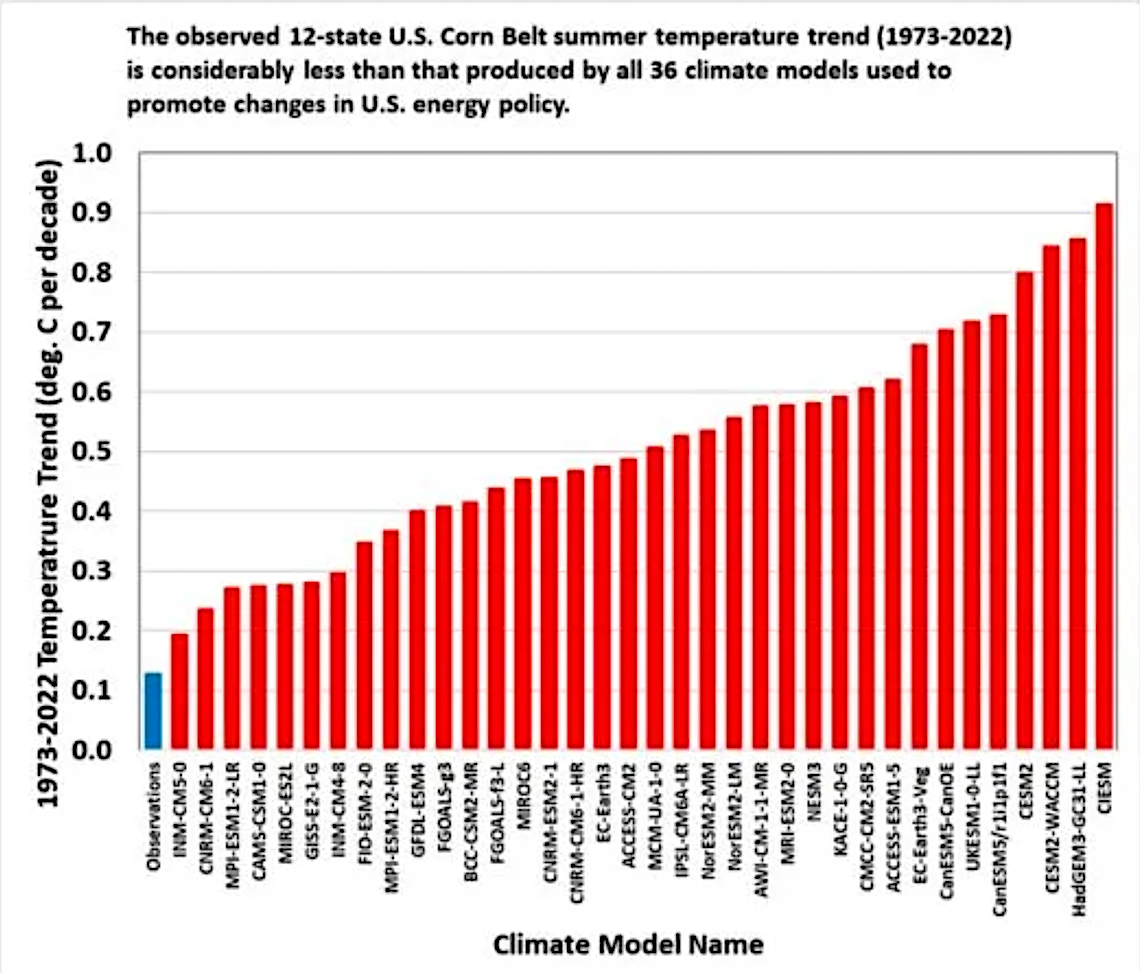
\includegraphics[width=4in]{../pics/climatemodels.png}
%
%Are climate models which vastly overstate temperature increases in correspondence with actuality?

\pn Engineering truth\index{engineering truth}  is different from scientific truth, even though we apply identical theories of physics, chemistry, and materials.  Engineering truth is also different from mathematical truth, even though we use mathematical understanding of matter and energy to bend it to human will.
\emph{Engineers make it so.}  As part of the design process, engineers make models which are in some way abstractions of the product to be sold to customers.  An abstraction attempts to accurately represent some aspects of the product, and ignore the rest.  Engineers \emph{create} truth.

\pn Engineers \comment{(will)} use SysML to create models (abstractions) of systems in the process of designing the systems to correspond with the models.
Thus engineering truth is vastly stronger than scientific truth because engineers get to make both the abstraction and the actuality.

\pn To the extent that models and specifications can be mathematically precise, correctness can approach the ultimate:  mathematical truth.

\begin{quotation}
First-order Zermelo-Fraenkel set theory is widely regarded as the standard of mathematical correctness, in the sense that a proof is correct if and only if it can be formalized as a deductive proof in set theory.\cite{tarski-truth}
\end{quotation}

\pn These metaphysics establish the grounds so that system models can be constructed and analyzed using first-order classical logic and set theory to attain the highest form of mathematical truth.

\section{Formality}\label{sec:formality}

\gloss{formal}{Relating to or involving outward form or structure, often in contrast to content or meaning.}

\gloss{semantics}{Definition of meaning.}

\pn To be \bemph{formal} is to have \bemph{form}.  Having form allows definition of meaning or \bemph{semantics}.

\gloss{formula}{Formal sentence.}

\pn A well-formed formula (WFF)\index{WFF} can have meaning.  Poorly formed formulas are meaningless.  

\pn Given a collection of facts (WFFs) known or assumed to be true, other true facts (WFFs) can be derived by sound inference rules.  Such inference rules depend on the \emph{form} of wffs--not their content.
This allows generality in application of inference rules to derive new (true) facts from known (true) facts.

\gloss{material implication}{$(p\rightarrow q)$ is true whenever $p$ is false or $q$ is true.}

\pn Suppose we know fact (WFF) $A$ is true, and that $A$ materially implies $B$, $(A\rightarrow B)$.  Then applying the \bemph{modus ponens} inference rule, we can deduce that $B$ is also true, regardless of the specific facts $A$ and $B$.

\gloss{modus ponens}{If $p$ and $(p\rightarrow q)$, then $q$.}

\pn Adherents of relevance logic \cite{sep-logic-relevance} would complain that the conclusion of implication, $B$, need have nothing to do with the premise $A$.  Nevertheless, we declare the 

\gloss{Fundamental Principle of Systems Engineering Metaphysics}{Semantics requires formality for specificity.}

\pn Informal semantics can be ambiguous or misinterpreted.  For SysML models to have exactly the same meaning for analysis, verification, testing and deployment, language semantics must be formal.

\subsection{Metamath}\label{sec:metamath}

\pn Formality is defined in terms of Metamath.

\pn \bemph{Metamath} is the name of a language for expressing theorems and proofs (see Appendix \ref{chapter:metamath}).  
Metamath is also the name of a checker for proofs expressed in the Metamath language, and a website (\texttt{metamath.org}).  
\bemph{Metamath Proof Explorer} is the name of a particular database of theorems and proofs called \texttt{set.mm} derived from the axioms of classical (first-order) logic
and Zermelo-Fraenkel with Choice (ZFC) set theory.

\pn There are other databases which use different sets of axioms.  In particular, \texttt{iset.mm} uses intuitionistic logic for which the Law of Excluded Middle does not hold.

\pn The Metamath language is entirely ASCII.  The Metamath program can produce equivalent LaTeX for definitions, theorems, and proofs.

\pn \texttt{set.mm}\index{set.mm} is an ever-growing database of theorems and proofs in an attempt to prove ``all''\footnote{There are also databases for Category Theory which is `too big' for ZFC, and Quantum Logic which is too weird.} of mathematics from the axioms of classical logic (Law of Excluded Middle holds)
and ZFC (Zermelo-Fraenkel with Choice) set theory.
\texttt{set.mm} holds  $>$30k axioms, definitions, and theorems with proofs.  Definitions must be expressed in restricted form so they can be eliminated by substitution so every theorem and proof can be reduced to the axioms.

\pn All of the definitions and theorems are defined either in Metamath directly, or in its style.

\subsection{Lean}\label{sec:lean}

\pn Lean provides a second, independent way to make the same formality machine-checkable.

\pn \bemph{Lean}\footnote{https://lean-lang.org} is the name of both a functional programming language and an interactive theorem prover (proof assistant) built on that language, originally created by Leonardo de Moura.  Lean is now in its fourth major revision, \bemph{Lean 4}, a complete reimplementation of the language and its kernel.

\pn Unlike Metamath, whose \texttt{set.mm} database is built on classical first-order logic and Zermelo-Fraenkel with Choice (ZFC) set theory, Lean's kernel implements a \bemph{dependent type theory} (a variant of the Calculus of Inductive Constructions).  Propositions are types, and proofs are programs of that type---the Curry--Howard correspondence.  A proof is accepted only when Lean's small, independently reimplementable \bemph{kernel} type-checks the corresponding program; everything built on top of the kernel (tactics, automation, elaboration, notation) exists only to construct that program, and is itself untrusted.

\pn \bemph{Mathlib}\index{Mathlib} is the community-maintained library of formalized mathematics for Lean 4, filling the same role \texttt{set.mm} fills for Metamath: a single, continually-growing, peer-reviewed collection of definitions and proved theorems, covering most of an undergraduate and much of a graduate mathematics curriculum, that later work can build on rather than re-derive.

\pn The Lean language is not restricted to ASCII the way the Metamath language is; source files are Unicode, so formulas can be written directly with symbols such as $\forall$, $\exists$, $\neg$, $\wedge$, and $\rightarrow$ rather than reserved ASCII tokens.

\pn This project maintains \texttt{SFS.lean}\index{SFS.lean}, an independent Lean 4/Mathlib translation of the same Domain Logic and Metaphysics content formalized in \texttt{SFS.mm} (Appendix \ref{chapter:mm}).  Where Metamath is used, as described above, to prove that BLESS's proof rules are sound from the axioms of classical logic and ZFC, \texttt{SFS.lean} independently re-derives---or, where a rule turns out not to be sound in general, exposes the failure with a counterexample---the same results from Lean's dependent type theory, so that a mistake specific to one formal system's encoding is unlikely to survive undetected in both.

\section{Ontology}\label{sec:ontology}
 
\pn In philosophy, \emph{ontology} is the study of being:  what is.
\gloss{philosophical ontology}{the study of being}

\pn In technology, \emph{ontology} defines classes of things and procedures for classification.
Technical ontology has been particularly successful in biology, chemistry, and information technology.
OWL (Web Ontology Language) \cite{OWL} is the most popular technical ontology language.
KerML \S 8.4.3 defines ontological semantics for Core-level elements by mapping (interpreting) elements them to sets of tuples.
\gloss{technological ontology}{classes and classification procedures}

\section{Modality}\label{sec:modality}

\gloss{modal}{Related to context.}

\pn Modal statements tell us something about what could be or must be the case.\cite{modality-varieties}
Consider:
\begin{enumerate}
\item No one can be both a bachelor and married. (‘Bachelor’ means ‘unmarried man’.)
\item You could not have been born of different parents. (Someone born of different parents wouldn’t be you.)
\item Nothing can travel faster than light. (It’s a law of nature.)
\item One cannot get from London to New York in less than one hour. (Planes that fast haven’t been built yet.)
\item You cannot leave the palace. (The doors are locked.)
\item You cannot promise to come and then stay at home. (It’s wrong.)
\item You cannot start a job application cover letter with “hey guys”. (It’s just not done.)
\item You cannot castle if your king is in check. (It’s against the rules.)
\item You cannot deduct your holidays from your taxes. (It’s against the law.)
\item Fred cannot be the killer. (The evidence shows that he’s innocent.)
\end{enumerate}

\pn Each of these claims appears to have a true reading. But it also seems that ‘cannot’ needs to be interpreted in different ways to make the different sentences true.

\pn The modal claims (1)–(10) appear to be true for completely different reasons. For example, it may be held that the truth of (1) is due to the meanings of its constituent expressions; that (2) holds because it lies in your nature to be born of your actual parents; that (3) is true because the laws of nature preclude superluminal motion; that (4) holds because of technological limitations; that (5) owes its truth to the presence of insurmountable practical obstacles; that (6)–(9) are made true by the demands of morality, etiquette, the rules of chess, and the law respectively; and that (10) holds because the known facts prove Fred’s innocence.

\pn It is one of the tasks of a philosophical theory of modality to give a systematic and unified account of this multiplicity of modal concepts.
For this philosophers employ the concept of \emph{possible worlds} providing distinct contexts or modes (hence `modal').

\pn The apparatus of possible worlds allows us to introduce a set of modal notions:  necessary, possible, contingent.
\gloss{necessary}{A proposition is true in all possible worlds.}
\gloss{possible}{A proposition is true in some possible worlds.}
\gloss{contingent}{A proposition is true in some but not all possible worlds.}

\pn One of the main purposes of language is to transmit information about the world. Where 
$P$
 is any sentence used for that purpose (roughly speaking, a declarative sentence), it seems natural to think of 
$P$’s content (the proposition expressed by it) as the information that is semantically encoded in it. Combining this with the foregoing account of information, we can think of the content of a sentence as a set of possible worlds (namely, the set containing just those worlds of which the sentence is true) or, equivalently, as a function from worlds to truth-values.  This is satisfaction.

\gloss{satisfaction}{Making a sentence/proposition/predicate true.}

\pn These concepts connect the modal, epistemic and semantic realms in a simple and elegant way.  

\pn Philosophers can endlessly elaborate \comment{(perhaps while dining)} by considering counterfactuals, whether designators are rigid, whether propositions are true by pure reason (a priori) of depend on known facts (a posteriori), or whether the proposition is mathematical, natural (physics), mental, or metaphysical.

\pn Fortunately, we are engineers seeking to establish engineering truths.  Therefore, we get to choose metaphysics for systems engineering which are appropriate and unambiguous.

\gloss{metaphysical necessity}{Conforming to these metaphysics, or derived from them by deductive proof.}

\gloss{nomic necessity}{Conforming to natural laws (physics, chemistry, etc.).}

System engineering metaphysics elides philosophical conundrums by metaphysical necessity.

\section{Physical and Virtual}\label{sec:phyeph}

\pn Machines are necessarily physical:  made of matter.  They are manufactured, assembled, transported, and stored.  Software and information are virtual and can be used only when allocated to something physical.

\pn Physical things necessarily have location, size/shape, mass, velocity, inertia, material, and much else.

\pn Virtual things have none of these attributes; to perform system functions they must be allocated to physical things like processors, memories, buses etc.

\pn Distinct physical things cannot occupy the same location at the same time, but a data structure (virtual) must co-locate with a memory (physical) to exist at all!

\pn Consequently, physical things and virtual things must be metaphysically different.  
\gloss{ontologically depends}{An entity would not exist without the other.}

\pn Virtual things ontologically depend on physical things.  Virtual things must be allocated to physical things.

\section{Spacetime}\label{sec:spacetime}

\pn Spacetime is modeled as frames-of-reference.  Each \bemph{frame-of-reference} has three spacial dimensions plus time.  Within a frame-of-reference space is rectilinear (does not curve and axises are perpendicular) and time moves forward uniformly.  

\subsection{Frames-of-Reference}\label{sec:frames}

\pn Most systems will occupy a single frame-of-reference. 
Consider a car's frame of reference having origin equidistant from the hubs of its wheels with its Y-axis toward the front, its X-axis towards the right side, and its Z-axis straight up.  Such a frame of reference could define the location of all the car's parts.  

DIAGRAM OF CAR FRAME-OF-REFERENCE HERE \comment{(get from Hans Peter)}

\pn To model driving the car, move the car's frame-of-reference relative to the road's frame of reference.

\pn Systems-of-systems (SoS) might need to be modeled with multiple \bemph{frames-of-reference}.  Consider an air-traffic control system or a Starlink constellation.  Relativistic effects such as time dilation due to velocity or space curvature due to mass would be modeled as relationships between multiple frames-of-reference.

\gloss{Principle of Relativity}{All inertial frames-of-reference are completely equivalent for the formulation of the Laws of Physics.}

\gloss{substantialism}{The view that spacetime has an existence independent of objects and processes occurring within it.}

\pn Our frames-of-reference presume the Principle of Relativity and substantialism.

\subsection{Time}\label{sec:fortime}

\pn Within a frame-of-reference, time is modeled separately from space.  Time will be modeled as a modal logic having different ``worlds" for each instant\index{instant} (a.k.a moment\index{moment}) of time.\index{time}  

\gloss{Newtonian spacetime}{The temporal interval between any two events is a well-defined quantity.}

\pn Our frames-of-reference presume Newtonian spacetime\cite{spacetime-bebecome}, which is another reason to prefer instant over interval as the fundamental model of time.\footnote{Switching from intervals to instants may seem traumatic, but won't be because intervals can be defined using instants, and can be open on one or both ends.  \texttt{middleTimeSlice} is the open interval between \texttt{startShot} and \texttt{endShot}.}

\gloss{simultaneous}{The temporal interval between two events is 0.}

\pn There are three metaphysics of time:  presentism, possibilism, and eternalism, Figure \ref{fig:3metaphysics}.

\begin{figure}[h]
\begin{center}
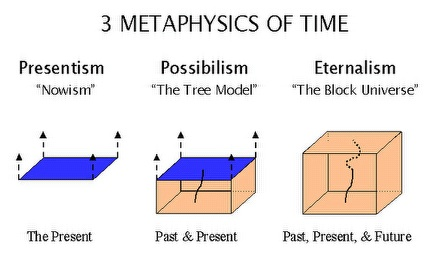
\includegraphics[width=5in]{../pics/3metaphysics}
\caption{Three Metaphysics of Time\cite{spacetime-bebecome}}
\label{fig:3metaphysics}
\end{center}
\end{figure}

\gloss{presentism}{Only the present exists.}
The diagram illustrating presentism has four arrows pointing towards the top of the page (conventionally taken to represent the future direction) attached to the plane representing the present. These arrows are meant to indicate something that is integral to presentism, the idea that the present (and hence the existent) constantly shifts or changes.

\gloss{eternalism}{Past, present, and future exist.}
With eternalism, there is nothing more special about the temporal present (the \emph{now}) than the spatial present (the \emph{here}). Future and past events at a place, on this view, are no more or less real than distant events at a time. 
The \emph{now} like the \emph{here} is a function of one’s perspective, one’s position in the spacetime, and these positions are indicated by the line in the spacetime representing the history of spacetime locations of a particular object or person.

\gloss{possibilism}{The future is possible; the past has become actual; the present we can affect.}

\pn We choose possibilism for our metaphysics with the added restriction of an initial time, $\tau=0$, at which the initial conditions are prescribed (known, set).
This lower boundary condition on time allows a definitive starting point for modeling the behavior of systems.  Our systems always act \bemph{now} based on current conditions and what has happened in the past. 

\section{Mereology}\label{sec:mereology}

\gloss{mereology}{Theory of parthood relations: of the relations of part to whole and the relations of part to part within a whole.\cite{mereology}}

\pn This section considers spatial mereology, parthood of \bemph{things} in space.  In our metaphysics, `things' are physical, occupy space and have mass.  There are no temporal parts of things because how things change over time is modeled using modal logic worlds.

\gloss{part}{Functional subunit.}

\pn Mereologies\footnote{There are different philosophical opinions for mereology.  That's why we explicitly define it in the context of systems engineering.} generally defines parthood reflexively:  anything is part of itself.  Our definition of \bemph{part} is what some mereologies call \bemph{proper part}.
An infix notation will be used to define axioms for $P$.  $xPy$ means $x$ is a (proper) part of $y$.  All quantification refers to things in a frame-of-reference.

\pn Nothing can be part of itself.
\begin{restatable}{metadefinition}{df-par}~\blTitle{df-par}~ Define part antireflexivity.
\begin{align}
\vdash \lnot x \,P \,x\label{eq:df-par}\tag{df-par}
\end{align}
\end{restatable}

\begin{restatable}{leandefinition}{parLean}~\leanTitle{par}~ Define part antireflexivity in Lean.

\texttt{\textcolor{leancolor}{axiom} \textcolor{leanyellow}{par} (x : Occurrence) : $\lnot$ PartOf x x}
\label{par}
\end{restatable}

\pn A part of a part is a part.
\begin{restatable}{metadefinition}{df-ptr}~\blTitle{df-ptr}~ Define part transitivity.
\begin{align}
\vdash ( ( x \,P \,y \wedge y \,P \,z ) \rightarrow x \,P \,z
    )\label{eq:df-ptr}\tag{df-ptr}
\end{align}
\end{restatable}

\begin{restatable}{leandefinition}{ptr}~\leanTitle{ptr}~ Define part transitivity in Lean.

\texttt{\textcolor{leancolor}{axiom} \textcolor{leanyellow}{ptr} \{x y z : Occurrence\} : PartOf x y $\to$ PartOf y z $\to$ PartOf x z}
\label{ptr}
\end{restatable}

\pn Having a part in common is called \bemph{overlap}, $xOy$.
\begin{restatable}{metadefinition}{df-pov}~\blTitle{df-pov}~ Define part overlap.
\begin{align}
\vdash x \,O \,y \leftrightarrow \exists z ( z \,P \,x \wedge z \,P \,y
    )\label{eq:df-pov}\tag{df-pov}
\end{align}
\end{restatable}

\begin{restatable}{leandefinition}{Overlap}~\leanTitle{Overlap}~ Define part overlap in Lean.

\texttt{\textcolor{leancolor}{def} \textcolor{leanyellow}{Overlap} (x y : Occurrence) : Prop := $\exists$ z, PartOf z x $\wedge$ PartOf z y}
\label{Overlap}
\end{restatable}

\pn Being parts of the same thing is called \bemph{underlap}, $xUy$.
\begin{restatable}{metadefinition}{df-pun}~\blTitle{df-pun}~ Define part underlap.
\begin{align}
\vdash x \,U \,y \leftrightarrow \exists z ( x \,P \,z \wedge y \,P \,z
    )\label{eq:df-pun}\tag{df-pun}
\end{align}
\end{restatable}

\begin{restatable}{leandefinition}{Underlap}~\leanTitle{Underlap}~ Define part underlap in Lean.

\texttt{\textcolor{leancolor}{def} \textcolor{leanyellow}{Underlap} (x y : Occurrence) : Prop := $\exists$ z, PartOf x z $\wedge$ PartOf y z}
\label{Underlap}
\end{restatable}

\pn Improper part is proper part or equal, $xIPy$.
\begin{restatable}{metadefinition}{df-pim}~\blTitle{df-pim}~ Define improper part
\begin{align}
\vdash x \,IP \,y \leftrightarrow ( x \,P \,y \vee x = y
    )\label{eq:df-pim}\tag{df-pim}
\end{align}
\end{restatable}

\begin{restatable}{leandefinition}{ImproperPart}~\leanTitle{ImproperPart}~ Define improper part in Lean.

\texttt{\textcolor{leancolor}{def} \textcolor{leanyellow}{ImproperPart} (x y : Occurrence) : Prop := PartOf x y $\vee$ x = y}
\label{ImproperPart}
\end{restatable}

\pn Having no part in common is called \bemph{disjoint}, $xDy$.
\begin{restatable}{metadefinition}{df-pdj}~\blTitle{df-pdj}~ Define part disjointness
\begin{align}
\vdash x \,D \,y \leftrightarrow \lnot x \,O \,y\label{eq:df-pdj}\tag{df-pdj}
\end{align}
\end{restatable}

\begin{restatable}{leandefinition}{PartDisjoint}~\leanTitle{PartDisjoint}~ Define part disjointness in Lean.

\texttt{\textcolor{leancolor}{def} \textcolor{leanyellow}{PartDisjoint} (x y : Occurrence) : Prop := $\lnot$ Overlap x y}
\label{PartDisjoint}
\end{restatable}

\pn In addition systems have a \bemph{containment hierarchy}.
Given any two things, either one is part of the other, they are disjoint, or they are the same, and they can't be parts of each other.
\begin{restatable}{metadefinition}{df-pch}~\blTitle{df-pch}~ Define part containment hierarchy.
\begin{align}
\vdash ( ( ( x \,P \,y \vee y \,P \,x ) \vee ( x = y \vee x \,D \,y ) ) \wedge
    \lnot ( x \,P \,y \wedge y \,P \,x ) )\label{eq:df-pch}\tag{df-pch}
\end{align}
\end{restatable}

\begin{restatable}{leandefinition}{pch}~\leanTitle{pch}~ Define part containment hierarchy in Lean. Despite the
\texttt{df-} name this doesn't define a new symbol --- it's purely a constraint not derivable from
\texttt{par}/\texttt{ptr} alone, so, like those two, it stays an axiom here too.

\texttt{\textcolor{leancolor}{axiom} \textcolor{leanyellow}{pch} (x y : Occurrence) :}

\texttt{~~((PartOf x y $\vee$ PartOf y x) $\vee$ (x = y $\vee$ PartDisjoint x y)) $\wedge$ $\lnot$ (PartOf x y $\wedge$ PartOf y x)}
\label{pch}
\end{restatable}

\pn A part is an \bemph{atom} if it has no parts itself, $Ax$.
\begin{restatable}{metadefinition}{df-pat}~\blTitle{df-pat}~ Define atomic part.
\begin{align}
\vdash A \,x \leftrightarrow \lnot \exists z ( z \,P \,x
    )\label{eq:df-pat}\tag{df-pat}
\end{align}
\end{restatable}

\begin{restatable}{leandefinition}{AtomPart}~\leanTitle{AtomPart}~ Define atomic part in Lean.

\texttt{\textcolor{leancolor}{def} \textcolor{leanyellow}{AtomPart} (x : Occurrence) : Prop := $\lnot$ $\exists$ z, PartOf z x}
\label{AtomPart}
\end{restatable}

\pn A \bemph{whole} has all things in a frame-of-reference as parts, except itself, $Wx$.
\begin{restatable}{metadefinition}{df-pwh}~\blTitle{df-pwh}~ Define whole.
\begin{align}
\vdash W \,x \leftrightarrow \forall z ( z \,P \,x \vee x = z
    )\label{eq:df-pwh}\tag{df-pwh}
\end{align}
\end{restatable}

\begin{restatable}{leandefinition}{WholePart}~\leanTitle{WholePart}~ Define whole in Lean.

\texttt{\textcolor{leancolor}{def} \textcolor{leanyellow}{WholePart} (x : Occurrence) : Prop := $\forall$ z, PartOf z x $\vee$ x = z}
\label{WholePart}
\end{restatable}

\pn Systems engineering requires mereological fusion.

\gloss{mereological fusion}{Parts become the whole; the whole supervenes the parts with metaphysical necessity.}

\gloss{supervenes}{A supervenes B if there cannot be an A-difference without a B-difference.}


\section{Location and Mereology}\label{sec:location-mereology}

\pn A \bemph{region} is a contiguous, three-dimensional volume at a particular place in a particular 
frame-of-reference.\cite{location-mereology}
Regions do not have parts.  A region may overlap or contain other regions.

\pn The \bemph{location} of a physical object is the region it occupies (within a frame-of-reference, at a particular moment of time).
Virtual objects have no location themselves, but obtain location secondarily when allocated to a physical object.

\pn The set of locations (of all things within a frame-of-reference, at a particular moment of time) is a relation, $xLr$, having
domain of things ($x~ y~ z$) and co-domain of regions ($r~ r_1~ r_2$).

\pn We take \bemph{exact location}, $xLr$, as our unique locative primitive. We assume that
\begin{enumerate}
\item it is a two-place relation, and
\item both argument places in that relation are singular.
\end{enumerate}

\pn But both (1) and (2) have been questioned.
For example, one might reject (1) in favor of the view that exact location is a three-place relation that holds between a located entity, a region of space, and an instant of time. This is a natural view for those who think of space as a three-dimensional entity that 
\bemph{endures} through, and is separate from, time.  We get that effect with temporal worlds.

\pn Alternatively, one might agree that exact location is a two-place relation but reject (2) above in favor of the view that, say, the second argument place in exact location (the ‘location’ slot) is plural.  This will be true of systems-of-systems where different subsystems occupy different frames-of-reference.  Consider a television and its remote control as a system-of-systems each having its own frame-of-reference, within which each part has fixed location.

\pn Nothing has more than one location (within a frame-of-reference, at a particular moment of time)\footnote{to be assumed henceforth unless explicitly stated otherwise}.  This principle is called \bemph{locational functionality}.
\begin{restatable}{metadefinition}{df-lfu}~\blTitle{df-lfu}~ Define locational functionality L.
\begin{align}
\vdash \forall x \forall r_1 \forall r_2 ( ( x \,L \,r_1 \wedge x \,L \,r_2 )
    \rightarrow r_1 = r_2 )\label{eq:df-lfu}\tag{df-lfu}
\end{align}
\end{restatable}

\begin{restatable}{leandefinition}{lfu}~\leanTitle{lfu}~ Locational functionality is now a real theorem, not an
axiom, in Lean: a Lean function is automatically single-valued, so \texttt{Location}'s own function-valued type
already proves it.

\texttt{\textcolor{leancolor}{theorem} \textcolor{leanyellow}{lfu} \{x : Occurrence\} \{r1 r2 : Region\} (h1 : Location x = r1) (h2 : Location x = r2) : r1 = r2 := h1 $\triangleright$ h2}
\label{lfu}
\end{restatable}

\pn No two things share an exact location.  This principle is called \bemph{injectivity of location}.
\begin{restatable}{metadefinition}{df-lin}~\blTitle{df-lin}~ Define injectivity of location.
\begin{align}
\vdash \forall x \forall y \forall r ( ( x \,L \,r \wedge y \,L \,r ) \rightarrow x =
    y )\label{eq:df-lin}\tag{df-lin}
\end{align}
\end{restatable}

\begin{restatable}{leandefinition}{lin}~\leanTitle{lin}~ Injectivity of location in Lean. Still a genuine,
non-derivable constraint even with \texttt{Location} function-valued (nothing forces a function to be
injective), so this stays an axiom.

\texttt{\textcolor{leancolor}{axiom} \textcolor{leanyellow}{lin} \{x y : Occurrence\} \{r : Region\} : Location x = r $\to$ Location y = r $\to$ x = y}
\label{lin}
\end{restatable}

\pn Two regions containing the same point \bemph{overlap}, $r_1Or_2$.  A region $r$ is a set of points, and {contains} point $p$
iff $p~\epsilon_r~ r$.
\begin{restatable}{metadefinition}{df-rov}~\blTitle{df-rov}~ Define region overlap O.
\begin{align}
\vdash r_1 \,O \,r_2 \leftrightarrow \exists p ( p ~\epsilon_r~ r_1 \wedge p
    ~\epsilon_r~ r_2 )\label{eq:df-rov}\tag{df-rov}
\end{align}
\end{restatable}

\begin{restatable}{leandefinition}{RegionOverlap}~\leanTitle{RegionOverlap}~ Define region overlap in Lean.

\texttt{\textcolor{leancolor}{def} \textcolor{leanyellow}{RegionOverlap} (r1 r2 : Region) : Prop := $\exists$ p, InRegion p r1 $\wedge$ InRegion p r2}
\label{RegionOverlap}
\end{restatable}

\pn A region \bemph{contains} another, $r_1Cr_2$ when it contains all of its points.
\begin{restatable}{metadefinition}{df-rco}~\blTitle{df-rco}~ Define region containment C.
\begin{align}
\vdash r_1 \,C \,r_2 \leftrightarrow \forall p ( p ~\epsilon_r~ r_2 \rightarrow p
    ~\epsilon_r~ r_1 )\label{eq:df-rco}\tag{df-rco}
\end{align}
\end{restatable}

\begin{restatable}{leandefinition}{RegionContainment}~\leanTitle{RegionContainment}~ Define region containment in Lean.

\texttt{\textcolor{leancolor}{def} \textcolor{leanyellow}{RegionContainment} (r1 r2 : Region) : Prop := $\forall$ p, InRegion p r2 $\to$ InRegion p r1}
\label{RegionContainment}
\end{restatable}

\pn A region is \bemph{atomic}, $Ar$, when it contains no other regions.
\begin{restatable}{metadefinition}{df-rat}~\blTitle{df-rat}~ Define atomic region.
\begin{align}
\vdash A \,r \leftrightarrow \forall r_1 ( r \,C
    \,r_1 \rightarrow r = r_1 )\label{eq:df-rat}\tag{df-rat}
\end{align}
\end{restatable}

\begin{restatable}{leandefinition}{AtomicRegion}~\leanTitle{AtomicRegion}~ Define atomic region in Lean.

\texttt{\textcolor{leancolor}{def} \textcolor{leanyellow}{AtomicRegion} (r0 : Region) : Prop :=}

\texttt{~~$\forall$ (x : Occurrence) (r1 : Region), Location x = r1 $\wedge$ RegionContainment r0 r1 $\to$ r0 = r1}
\label{AtomicRegion}
\end{restatable}

\pn No atomic regions overlap.
\begin{restatable}{metadefinition}{df-rdi}~\blTitle{df-rdi}~ Atomic regions are disjoint.
\begin{align}
\vdash \forall r_1 \forall r_2 ( ( A \,r_1 \wedge A \,r_2 ) \rightarrow ( \lnot r_1
    \,O \,r_2 \vee r_1 = r_2 ) )\label{eq:df-rdi}\tag{df-rdi}
\end{align}
\end{restatable}

\begin{restatable}{leandefinition}{rdi}~\leanTitle{rdi}~ Atomic regions are disjoint, in Lean.

\texttt{\textcolor{leancolor}{axiom} \textcolor{leanyellow}{rdi} \{r1 r2 : Region\} : AtomicRegion r1 $\to$ AtomicRegion r2 $\to$ $\lnot$ RegionOverlap r1 r2 $\vee$ r1 = r2}
\label{rdi}
\end{restatable}

\pn Atomic parts have atomic regions.
\begin{restatable}{metadefinition}{df-apar}~\blTitle{df-apar}~ Atomic parts have atomic regions.
\begin{align}
\vdash \forall x \forall r ( ( x \,L \,r \wedge A \,x ) \rightarrow A \,r
    )\label{eq:df-apar}\tag{df-apar}
\end{align}
\end{restatable}

\begin{restatable}{leandefinition}{apar}~\leanTitle{apar}~ Atomic parts have atomic regions, in Lean.

\texttt{\textcolor{leancolor}{axiom} \textcolor{leanyellow}{apar} \{x : Occurrence\} \{r0 : Region\} : Location x = r0 $\to$ AtomPart x $\to$ AtomicRegion r0}
\label{apar}
\end{restatable}

\pn Parthood implies regional containment.  This property is called \bemph{expansivity}.
\begin{restatable}{metadefinition}{df-pex}~\blTitle{df-pex}~ Define expansivity.
\begin{align}
\vdash \forall x \forall y \forall r_1 \forall r_2 ( ( x \,L \,r_1 \wedge y \,L
    \,r_2 \wedge x \,P \,y ) \rightarrow r_2 \,C \,r_1
    )\label{eq:df-pex}\tag{df-pex}
\end{align}
\end{restatable}

\begin{restatable}{leandefinition}{expansivity}~\leanTitle{expansivity}~ Define expansivity in Lean, tying
\texttt{PartOf} to \texttt{RegionContainment} via \texttt{Location}.

\texttt{\textcolor{leancolor}{axiom} \textcolor{leanyellow}{expansivity} \{x y : Occurrence\} \{r1 r2 : Region\} :}

\texttt{~~Location x = r1 $\to$ Location y = r2 $\to$ PartOf x y $\to$ RegionContainment r1 r2}
\label{expansivity}
\end{restatable}

\pn Regions overlap only if one contains the other.  This property is called \emph{no} \emph{interpenetration}.
\begin{restatable}{metadefinition}{df-rni}~\blTitle{df-rni}~ Define no interpenetration.
\begin{align}
\vdash \forall r_1 \forall r_2 ( r_1 \,O \,r_2 \rightarrow ( r_1 \,C \,r_2 \vee
    r_2 \,C \,r_1 ) )\label{eq:df-rni}\tag{df-rni}
\end{align}
\end{restatable}

\begin{restatable}{leandefinition}{noInterpenetration}~\leanTitle{no\_interpenetration}~ Define no
interpenetration in Lean.

\texttt{\textcolor{leancolor}{axiom} \textcolor{leanyellow}{no\_interpenetration} \{r1 r2 : Region\} : RegionOverlap r1 r2 $\to$ RegionContainment r1 r2 $\vee$ RegionContainment r2 r1}
\label{no_interpenetration}
\end{restatable}

\pn These choices for mereological metaphysics are called \bemph{supersubstantivalism} which entails perfect \bemph{mereolological harmony}.\cite{location-mereology}

\subsection{Surface and Interior}

\pn The definition of a region's \bemph{surface} and \bemph{interior} are necessarily defined together.  A region's surface are those point in a region ``adjacent'' to points not in the region.  A region's interior is all the points of a region not on its surface. Every point in a region is either in its interior, or on its surface, but not both.  A region's \emph{film} are those points adjacent to a region's surface, but not part of the region.

\pn The points \emph{adjacent} to a particular point are those whose distance to it approaches zero.  Let $D(p_1,p_2)$ be the distance between $p_1$ and $p_2$.\footnote{I'm unhappy with this definition of adjacent points, and welcome suggestions for improvement.}
\begin{restatable}{metadefinition}{df-adjp}~\blTitle{df-adjp}~ Define adjacent points.
\begin{align}
\vdash \textit{Adj}(p_1)~=~ \{~p_2~\vert~D(p_1,p_2) = d \wedge \lim_{d \to 0} d~\}
\label{eq:df-adjp}\tag{df-adjp}
\end{align}
\end{restatable}

\begin{restatable}{leandefinition}{Adjacent}~\leanTitle{Adjacent}~ Define adjacent points in Lean, as a
two-place predicate on points directly rather than translating \texttt{Adj}$(p_1)$'s set-builder form. No
further constraint (symmetry, irreflexivity, ...) is asserted beyond that.

\texttt{\textcolor{leancolor}{axiom} \textcolor{leanyellow}{Adjacent} : Point $\to$ Point $\to$ Prop}
\label{Adjacent}
\end{restatable}

\pn The surface of a region is points adjacent to points not in the region.

\begin{restatable}{metadefinition}{df-rsurf}~\blTitle{df-rsurf}~ Define surface of region.
\begin{align}
\vdash \textit{Surf}(r)~=~ \{~p~\vert~p~\epsilon_r~r~\wedge~\exists p_2~\vert~ p_2~\in~\textit{Adj}(p)~\wedge~\lnot p_2 ~\epsilon_r~r \}
\label{eq:df-rsurf}\tag{df-rsurf}
\end{align}
\end{restatable}

\begin{restatable}{leandefinition}{RegionSurface}~\leanTitle{RegionSurface}~ Define surface of region in Lean.
Function-valued (\texttt{Region} $\to$ \texttt{Surface}), matching \texttt{Regions.kerml}'s own functional
declaration: genuinely new content, asserting for the first time that every region has exactly one surface.

\texttt{\textcolor{leancolor}{axiom} \textcolor{leanyellow}{RegionSurface} : Region $\to$ Surface}

\texttt{\textcolor{leancolor}{axiom} \textcolor{leanyellow}{regionSurfaceProp} (r0 : Region) :}

\texttt{~~$\exists$ r1 : Region, $\forall$ p, OnSurface p (RegionSurface r0) $\to$ InRegion p r0 $\wedge$ $\lnot$ InRegion p r1}
\label{RegionSurface}
\end{restatable}

\pn The interior of a region is points not on its surface.

\begin{restatable}{metadefinition}{df-rint}~\blTitle{df-rint}~ Define interior of region.
\begin{align}
\vdash \textit{Rint}(r)~=~ \{~p~\vert~p~\epsilon_r~r~\wedge~p~\notin~\textit{Surf}(r) \}
\label{eq:df-rint}\tag{df-rint}
\end{align}
\end{restatable}

\begin{restatable}{leandefinition}{RegionInterior}~\leanTitle{RegionInterior}~ Define interior of region in Lean.
Function-valued (\texttt{Region} $\to$ \texttt{Region}) for the same reason as \texttt{RegionSurface} above.

\texttt{\textcolor{leancolor}{axiom} \textcolor{leanyellow}{RegionInterior} : Region $\to$ Region}

\texttt{\textcolor{leancolor}{axiom} \textcolor{leanyellow}{regionInteriorProp} (r1 : Region) :}

\texttt{~~$\forall$ p, InRegion p r1 $\to$ InRegion p (RegionInterior r1) $\wedge$ $\lnot$ OnSurface p (RegionSurface (RegionInterior r1))}
\label{RegionInterior}
\end{restatable}

\pn The film of a region is points not in the region, but adjacent to a point on its surface.

\begin{restatable}{metadefinition}{df-rfilm}~\blTitle{df-rfilm}~ Define film of region.
\begin{align}
\vdash \textit{Rfilm}(r)~=~ \{~p~\vert~\lnot~p~\epsilon_r~r~\wedge~\exists~p_2\vert~p_2~\in~\textit{Surf}(r)~\wedge~p_2~\in~\textit{Adj}(p)~ \}
\label{eq:df-rfilm}\tag{df-rfilm}
\end{align}
\end{restatable}

\begin{restatable}{leandefinition}{RegionFilm}~\leanTitle{RegionFilm}~ Define film of region in Lean. Needs no
new axiom: once \texttt{RegionSurface}/\texttt{RegionInterior} are functions, the film of \texttt{r0} is
already fully determined.

\texttt{\textcolor{leancolor}{noncomputable def} \textcolor{leanyellow}{RegionFilm} (r0 : Region) : Surface := RegionSurface (RegionInterior r0)}
\label{RegionFilm}
\end{restatable}

\subsection{Region Connection}

The Region Connection Calculus \cite{RCC8} consists of 8 basic relations that are possible between two regions.  Of these externally connected (EC) is most useful.  Two regions are externally connected if they ``touch'', having no points between, but don't overlap.  EC is used to define \texttt{Occurrences::JustOutsideOf}.


\begin{restatable}{metadefinition}{df-rec}~\blTitle{df-rec}~ Define external connection of regions.
\begin{align}
\vdash \textit{EC}(r_1,r_2)~\leftrightarrow~\lnot~r_1~O~r_2~\wedge~\exists~p~\vert~p~\in~\textit{Rfilm}(r_1)~\wedge~p~\epsilon_r~r_2
\label{eq:df-rec}\tag{df-rec}
\end{align}
\end{restatable}

\begin{restatable}{leandefinition}{ExternallyConnected}~\leanTitle{ExternallyConnected}~ Define external
connection of regions in Lean.

\texttt{\textcolor{leancolor}{def} \textcolor{leanyellow}{ExternallyConnected} (r1 r2 : Region) : Prop :=}

\texttt{~~$\exists$ p : Point, OnSurface p (RegionSurface r1) $\wedge$ OnSurface p (RegionSurface r2)}
\label{ExternallyConnected}
\end{restatable}




\section{Perdurance vs. Endurance}\label{sec:pervend}

\pn The debate over persistence of material objects through time centers around two rival views, endurantism and perdurantism.  Endurantists often say that a persisting material object is temporally unextended and in some sense ‘wholly present’ at each instant of its lifetime. Perdurantists often say that a persisting material object is a temporally extended entity that has a different temporal part at each different instant of its career and is at most partially present at any one instant.\cite{location-mereology}

\gloss{perdurance}{There are persisting material objects, and each such object has a different temporal part at each different instant at which the object exists.}

\gloss{endurance}{There are persisting material objects, but none of them has a different temporal part at each different instant of its career.}

\pn Choosing endurantism and relegating time to modal logic worlds circumvents contradictions and confusions.

\section{Sets}\label{sec:metasets}

\pn Almost any mathematical object can be viewed as a set, or a class (collection defined by a formula). The properties of the object can then be expressed in the language of set theory. A mathematical statement can be formalized into the language of set theory, and any mathematical theorem can be derived, using the calculus of classical first-order logic, from the axioms of Zermelo-Fraenkel with Choice (ZFC), or from some extension of ZFC. It is in this sense that set theory provides a foundation for mathematics.\cite{set-theory}

\pn The remarkable fact that virtually all of mathematics can be formalized within ZFC, makes possible a mathematical study of mathematics itself. Thus, any questions about the existence of some mathematical object, or the provability of a conjecture or hypothesis can be given a mathematically precise formulation. This makes metamathematics possible, namely the mathematical study of mathematics itself. So, the question about the provability or unprovability of any given mathematical statement becomes a sensible mathematical question. When faced with an open mathematical problem or conjecture, it makes sense to ask for its provability or unprovability in the ZFC formal system. Unfortunately, the answer may be neither, because ZFC, if consistent, is incomplete.

\pn Set theory and metamathematics are considered in sections \ref{sec:informal_sets} and \ref{sec:sets}.

\section{Particularity}\label{sec:particularity}

\pn Our models need to distinguish a particular thing (haecceity), a set of similar things (quiddity), and an element or elements of a set.  

\gloss{haecceity}{Aspects of a thing which makes it a particular thing (thissness).}

\gloss{quiddity}{Universal qualities of a thing which may be shared with other things, which may define a class/category/genus of things.}

\pn Usually when referring to elements of a set, the elements must be \bemph{distinct}.  To say that a car has four wheels, we mean that the car has four different wheels.  This combines quiddity (they're all wheels) with haecceity (they're different wheels).

\pn When defining multiplicity, distinctness is presumed.  Also, multiplicity should not be misused to make a set containing a single element, when what really needed is just the single element.


\section{Events and States}\label{sec:events}

\pn Events themselves are not things; they represent changes to things.  Such changes may cause things to exist, or cease to exist, or may change the properties of things.

\gloss{event}{Change occurring at a moment of time to (properties of) things which occur in space and time.}

\pn Similarly, states are not things; they represent the time between events when things remain the same.

\gloss{state}{Durations between events during which (properties of) things don't change.}

\pn Consider a door having four states:  open, closed, opening, and closing.  The event start-to-open is the transition from the closed to opening state.  While opening, the position of the door changes, but its property (moving from closed to open) remains the same.

\pn Some philosophers distinguish \emph{dynamic} from \emph{static} events \cite{sep-events}.  Here we consign static events to states.
Other philosophers consider negative events:  the dog did not bark during the night.  We only consider positive events.  The effect of negative events can be expressed as quantification over intervals:  there did not exist a time during the night at which the dog barked.

\pn Two events are the same if they are the same (identity) at the same moment of time (haecceity).  Of course, different events may occur at the same time.

\section{Causation}\label{sec:causation}

\pn Causation has been a vexatious topic in philosophy, some denying that there are any causal relations at all! \cite{sep-causation-metaphysics}  
Systems engineers know that this is nonsense.  Our systems are designed, built, bought, and used to \emph{do} something; systems are inherently causal.

\pn Metaphysically, causation is divided into four categories depending on the subject (tokens or types) and the effect (constant or variable).
A token is an individual thing (haecceity); a type is a category of things (quiddity).  A constant effect depends on existence or nonexistence; a variable effect depends on properties of things.

\begin{table}[h]
\caption{Causation Kinds}
\begin{center}
\begin{tabular}{|c|c|c|}
\hline
~ & \emph{Tokens} & \emph{Types} \\ \hline
\emph{Constants} & Token Causation & Type Causation \\ \hline
\emph{Variables} & Token Influence & Type Influence \\ \hline
\end{tabular}
\end{center}
\label{table:causation}
\end{table}%

\paragraph{Token Causation:}~~(1) The drought caused the famine.
\paragraph{Type Causation:}~~(2) Drowsy driving causes crashes.
\paragraph{Token Influence:}~~(3) How much I water my plant influences how tall it grows.
\paragraph{Type Influence:}~~(4) How much novocaine a patient receives affects how much pain they will feel during dentistry.

\pn A \bemph{token} can be an event, or a state, generalized as a \bemph{happening}.  The tokens of statement (1) are both states.
A \bemph{type} is a class of tokens.  In statement (2), `drowsy driving' is a class of states, while `crashes' is a class of events.
A \bemph{causation} relates existence.  Both statements (1) and (2) relate existence of things.
An \bemph{influence} relates variables (or properties).  In statement (3) the token is `my plant' with variables `water' and `tall'.
In statement (4), `a patient' selects an element of a type (implicitly applying to any and all elements of the type), for which `novocaine' and `pain' are variables.

\pn For the purposes of system operation, actions are always events, which always happen now (token causation).  However, our designs must define actions applied by any deployed systems in a range of circumstances (type causation).  Similarly for variable properties (token/type influence).  Though triggered by events, actions may have background or enabling conditions.

\pn A commonsensical idea about causation is that causal relationships are relationships that are potentially exploitable for purposes of manipulation and control: very roughly, if C
 is genuinely a cause of E, then if I can manipulate C in the right way, this should be a way of manipulating or changing E. \cite{sep-causation-mani}  This is the \bemph{manipulability} theory of causality, which is obviously applicable to systems engineering.
 Fortunately, our causality side steps issues with free actions, interventions, and counterfactuals.
 
 \subsection{Casual Models}\label{sec:causalmodels}
 
% Needed?  \cite{sep-causal-models} ``actual'' causation

\pn A \bemph{structural equation model} (SEM) characterizes a causal system with a set of variables, and a set of equations describing how each variable depends upon its immediate causal predecessors.\cite{sep-causal-models}  The variables represent the states of system elements.  For deterministic SEMs, variable values are typically natural numbers which encode enumeration literals expressing states of entities.
\gloss{SEM}{Structural Equation Model defining causality between states or events.}

\pn Consider a gas grill, used to cook meat. We can describe the operations of the grill using the following variables:
\begin{itemize}
\item Gas connected (1 if yes, 0 if no)
\item Gas knob (0 for off, 1 for low, 2 for medium, 3 for high)
\item Gas level (0 for off, 1 for low, 2 for medium, 3 for high)
\item Igniter (1 if pressed, 0 if not)
\item Flame (0 for off, 1 for low, 2 for medium, 3 for high)
\item Meat on (0 for no, 1 for yes)
\item Meat cooked (0 for raw, 1 for rare, 2 for medium, 3 for well done)
\end{itemize}
Thus, for example, Gas knob = 1 means that the gas knob is set to low; Igniter = 1 means that the igniter is pressed, and so on. Then the SEM equations might be:

Gas level = Gas connected $\times$ Gas knob \\
Flame = Gas level  $\times$ Igniter \\
Meat cooked = Flame  $\times$ Meat on \\

\pn The last equation, for example, tells us that if the meat is not put on the grill, it will remain raw (Meat cooked = 0). If the meat is put on the grill, then it will get cooked according to the level of the flame: if the flame is low (Flame = 1), the meat will be rare (Meat cooked = 1), and so on.

\pn A SEM is \emph{acyclic} if the variables can be ordered so that variables never appear on the left hand side of an equation after they have appeared on the right.  We will call an assignment of values to the exogenous variables a \emph{context}. In an acyclic SEM, a context uniquely determines the values of all the variables in the model.

%Deterministic SEMs naturally give rise to a logic of counterfactuals.
%\gloss{counterfactual}{Proposition in the form of a subjunctive conditional where the antecedent posits some circumstance, typically one that is contrary to fact.}
%Such counterfactuals applied to SEMs are called \bemph{interventions}.  `What if' the gas was not connected?  Then the meat would be raw.
%
%We interpret the counterfactual conditional $A\boxright B$ as saying that B would be true, if A were made true by an intervention.  However, $A$ must be plain boolean; $A$ cannot itself contain a counterfactual.  
%
%Counterfactuals are always considered in a context often called a `world'.  The antecedent of a counterfactual, $A$ is the intervention, or change in values of a world, even if the antecedent is already true in a given world.
%
%Supplement 1 of \cite{sep-causal-models} presents Briggs' axiomatization of structural counterfactuals.

\subsection{Other Terms}

\gloss{de re}{Relating to the properties of things mentioned in an assertion or expression, rather than to the assertion or expression itself.}
\gloss{de dicto}{Relating to the form of an assertion or expression itself, rather than any property of a thing it refers to.}
\gloss{factive}{Denoting a verb that assigns the status of an established fact to its object (normally a clausal object).}
\gloss{veridical}{Truthful, coinciding with reality.}
%\gloss{}{}
We strive to create veridical models.

\section{``M'' Levels}\label{sec:mlevels}

\pn Levels of abstraction are expressed with ``M'' levels, with the lowest abstraction, M0, corresponds to system operation in the field.


\begin{description}
\item[M0] - things being used (executed)
\item[M1] - model created by systems engineer
\item[M2] - metamodel, semantics, logic formulas (predicates)
\item[M3] - correctness proofs, many-world modal logic, ZFC, classical logic
\end{description}

\pn M0 objects are \bemph{instances}, and may be different in other temporal ``worlds'' corresponding to instants of time.  M0 is an abstraction of system operation--an execution model.%\footnote{Richard Page refers to the actual operation of a physical system as "M-1".}

\pn M1 objects are the SysML or KerML entities, in text or graphics, created by the system engineer.  M1 objects are represented as ZFC classes,\footnote{ZFC classes are different from the KerML entity.} collections defined by a rule.  M0 instances are elements of M1 classes.

\pn M2 objects are abstract syntax structures which impose constraints and define semantics using logic formulas in semantic metadata.
M2 objects define the rules used by M1 classes.

\pn M3 objects are theorems and proofs.  Proofs are sequences of theorems each of which is given or axiomatic, or is derived from prior theorems in the list by a sound inference rule.  Theorems are triples of M2 logic formulas.  Logics which apply to ordinary things are called first-order.  Logics which apply to formulas in different logics are called second-order.  Therefore the reasoning embodied in deductive behavior correctness proofs is second-order.

\pn Don't get hung up on ``M'' levels.  Each level of abstraction corresponds (or controls) to objects in the next lower level.
That's how correctness proofs of level M3, claim that every possible M0 execution conforms to its (behavioral) specification in M1.






